% You should title the file with a .tex extension (hw1.tex, for example)
\documentclass[a4paper, 11pt]{article}

\usepackage{amsmath}
\usepackage{amssymb}
\usepackage{fancyhdr}
\usepackage{graphicx}

\usepackage[margin=1in]{geometry}

\newcommand{\question}[2] {\vspace{.25in} \hrule\vspace{0.5em}
\noindent{\bf #1: #2} \vspace{0.5em}
\hrule \vspace{.10in}}
\renewcommand{\part}[1] {\vspace{.10in} {\bf (#1)}}

\newcommand{\myname}{Natthakan Euaumpon}
\newcommand{\myemail}{natthakaneuaumpon@gmail.com}
\newcommand{\myhwnum}{22}

\setlength{\parindent}{0pt}
\setlength{\parskip}{5pt plus 1pt}
 
\pagestyle{fancyplain}
\lhead{\fancyplain{}{\textbf{HW\myhwnum}}}      % Note the different brackets!
\rhead{\fancyplain{}{\myname\\ \myemail}}
\chead{\fancyplain{}{ICCS310 }}

\begin{document}

\medskip                        % Skip a "medium" amount of space
                                % (latex determines what medium is)
                                % Also try: \bigskip, \littleskip

\thispagestyle{plain}
\begin{center}                  % Center the following lines
{\Large ICCS310: Assignment \myhwnum} \\
\myname \\
\myemail \\
March 2020 \\
\end{center}

\question{1}{Lecture 22}
We already know that 3-SAT is in NP-Complete.\\
Assume that the 3-SAT problem has a 3-SAT formula of m clauses on n variables. Where $n$ variables is denoted by $x_1, ..., x_n$. Then we can construct a graph by:
\begin{enumerate}
	\item For every $x_i$ we create a vertex $v_i$ which will work as a negation of $x_i$
	\item For each clause c in $m$ add 5 vertices
	\item Three vertices of different colors are then added to denote the values True, False, and Base
	\item Add edges between the True, False and Base to form a triangle
	\item add edges among the vertices and the Base
\end{enumerate} 
Constraint of graph to make it True:
\begin{enumerate}
	\item For each pair of vertices they shouldnot be assign to the same value
	\item For each clause $c$ in $m$ at least one of the literal should hold True.
\end{enumerate}
Example would be:\\
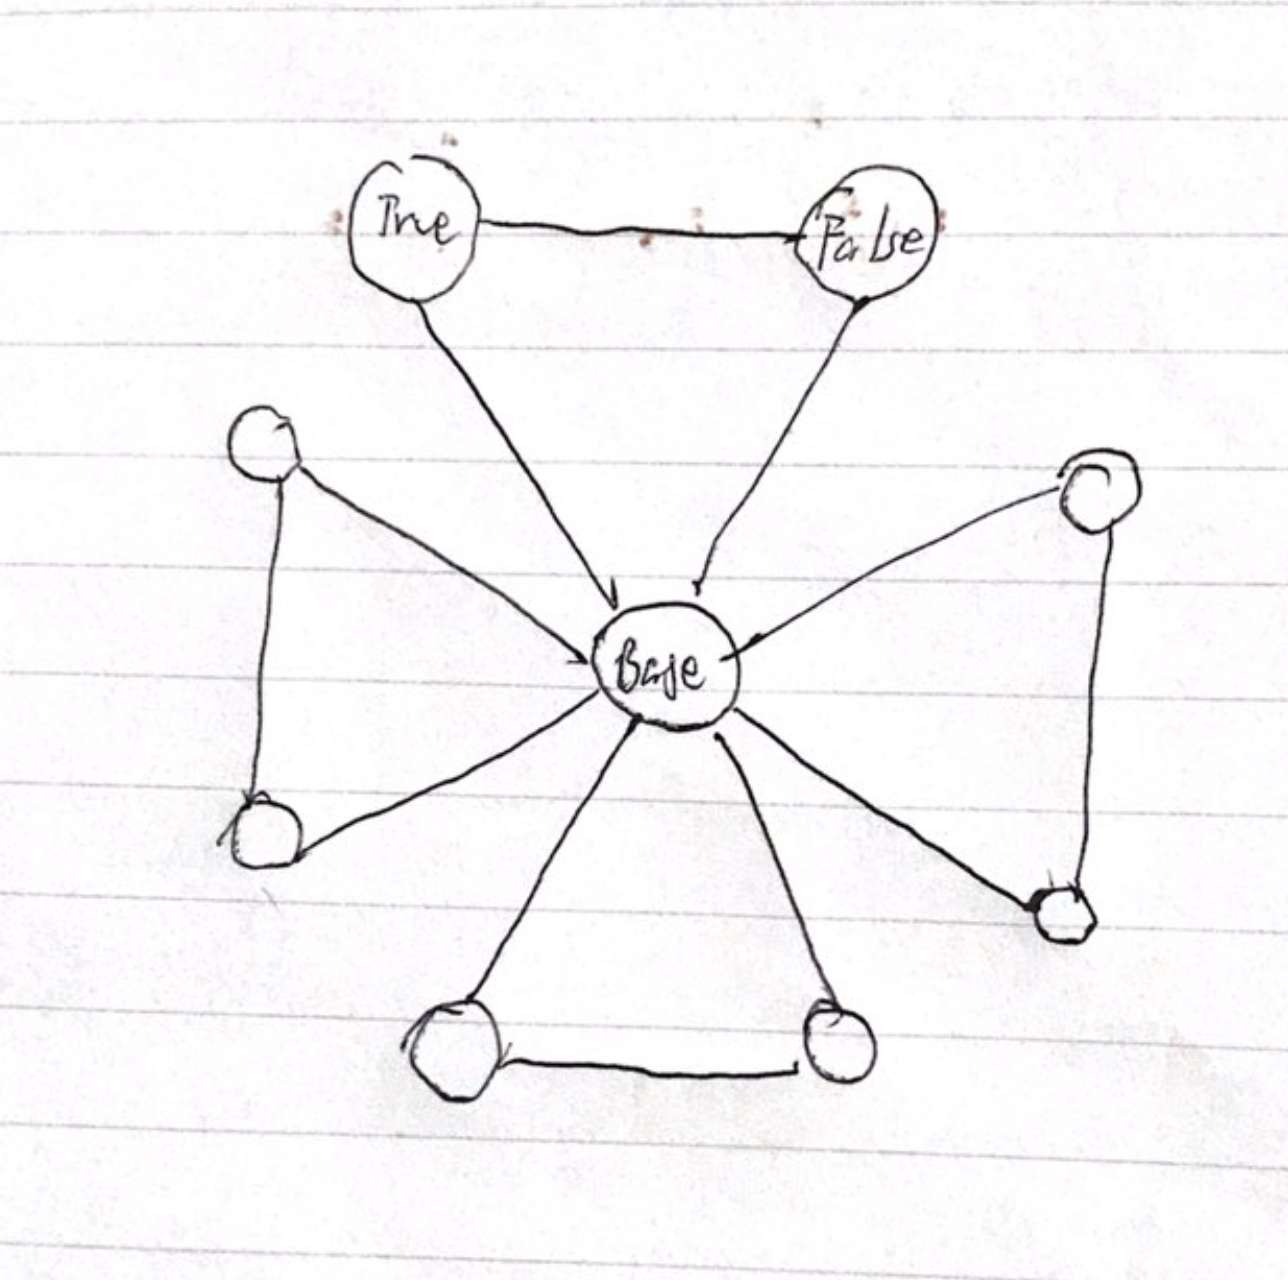
\includegraphics[width=\textwidth]{Q22.png}\\
WLOG, assume that this is satisfiable. Then for every clause atleast one of the literals $x_i$ must be true, therefore the corresponding $v_i$ will be assign True and $v_i^{'}$ will be False. Hence the graph can be 3 coloured. Consider that the graph is 3-colorable, so if the vertex $v_i$ is assigned to the True color, the coressponding variable $x_i$ will be True. This will form a truth assignment. Hence 3-coloring is NP-Complete.

\end{document}

